\ifdefined\included
\else
\documentclass[a4paper,11pt,twoside]{StyleThese}
\include{formatAndDefs}
% fallback si compilation standalone
\providecommand{\acs}[1]{#1}
\providecommand{\minitoc}{}
\providecommand{\dominitoc}{}
\providecommand{\faketableofcontents}{}
\usepackage{subcaption}
\hbadness=10000
\sloppy

\begin{document}
\setcounter{chapter}{2} %% Numéro du chapitre précédent ;)
\dominitoc
\faketableofcontents
\fi

\chapter{Détection d’anomalie multi-domaines}
\minitoc

%PB1 : Les méthodes proposées actuellement pour la détection d’anomalie sont pas adaptés
Le passage aux réseaux 5G s’accompagne d’un changement de paradigme majeur, caractérisé par une architecture distribuée et une complexification des interactions entre entités. Par ailleurs, l’émergence d’anomalies sémantique, séquentielle et topologique impose de nouvelles exigences en matière d’analyse. Dans ce contexte, il devient nécessaire non seulement d’adopter une analyse fine au niveau des paquets, mais également de prendre en compte le contexte dans lequel s’inscrivent les échanges. Or, cette problématique reste relativement récente dans le domaine des télécommunications, et les méthodes actuelles de détection d’anomalies apparaissent inadaptées à ce nouveau paradigme.

%PB2 : Pourquoi la formalisation de notre problème en GNN Dynamique nous parait pertinent
Dans ce contexte, nous proposons de représenter les échanges au sein des réseaux 5G sous la forme d’un graphe dynamique, permettant de capturer à la fois les interactions entre les différentes entités du réseau ainsi que l’évolution de ces interactions dans le temps. ette formalisation nous permet d’exploiter des techniques issues du domaine des GNN intrinsèquement adaptées à l’analyse des interactions complexes. Nous nous intéressons plus particulièrement aux GNN dynamiques, qui intègrent nativement la dimension temporelle.

%PB3 : Pourquoi le NLP est une bonne piste si on veut traiter une quantité indénombrable de données mais on ne l’a pas creusé

\section{Objectifs et cadre de détection}
% Scope = trafic de contrôle
Dans ces travaux, nous nous plaçons du point de vue de l’opérateur d’un réseau 5G et nous nous intéressons à la détection d’anomalies en nous concentrant exclusivement sur le trafic de contrôle échangé entre les entités du réseau, qu’il s’agisse du cœur de réseau ou du RAN. Le trafic utilisateur n’est pas pris en compte, car il ne présente pas de spécificités propres à l’architecture 5G et ne relève pas de la responsabilité directe du fournisseur d'accès réseau.

% Accès à tout le trafic
En se plaçant du point de vue de l’opérateur, nous supposons que celui-ci possède l’ensemble des NF et dispose d’un accès complet au trafic de contrôle. Dans l’architecture 5G, la fonction Service Communication Proxy (SCP) agit comme un intermédiaire dans les échanges entre les différentes NF, notamment pour le routage des requêtes et la vérification des autorisations d’accès. Dans ce contexte, il est raisonnable de considérer que l’opérateur peut observer l’intégralité du trafic de contrôle en déployant des sondes au niveau des SCP, qui constituent des points d’observation privilégiés des interactions entre NF. 

% Chiffrement
Ce trafic est généralement chiffré, par exemple via TLS sur le SBI ou via IPsec pour certains canaux, tels que N3 ou N4, reposant sur des protocoles spécifiques à la 5G. Cependant, en adoptant le point de vue de l’opérateur, nous supposons disposer des clés de chiffrement nécessaires pour accéder au contenu de ces échanges en clair.

% Performances
L’objectif serait de pouvoir exécuter nos modèles de détection en temps réel. Malgré les débits élevés offerts par la 5G, le volume de données est majoritairement porté par le trafic utilisateur, qui n’entre pas dans le périmètre de cette étude. À l’inverse, le trafic de contrôle est principalement composé de messages liés aux changements d’état des entités du réseau, qu’il s’agisse d’UE ou de NF, et ont une fréquence d’occurrence plus modérée. Par conséquent, bien que le surcoût induit par nos modèles puisse avoir un impact sur les performances, il est raisonnable de supposer que les ressources disponibles sont suffisantes pour permettre un traitement en temps réel, notamment grâce à l’exploitation de techniques d’optimisation et de parallélisation.

% Remédiation
La remédiation des anomalies détectées ne relève pas du périmètre de ce travail et est considérée comme une brique fonctionnelle distincte. Nous nous concentrons exclusivement sur la détection et les alertes générées par notre système ont vocation à être exploitées de manière similaire à celles produites par un système de détection d’intrusion (IDS) classique. Elles peuvent ainsi conduire, par exemple, à des ajustements des règles de firewall ou à des modifications de l’architecture réseau.

% Vrais objectifs
L’objectif de ces travaux n’est pas de concevoir un système de détection absolu et entièrement autonome. En effet, une anomalie ne constitue pas nécessairement le signe d’une activité malveillante et peut résulter d’une mise à jour, d’une erreur de configuration ou encore d’une interconnexion avec un système tiers, comme dans le cas du roaming. Dans ce contexte, la distinction entre une anomalie bénigne et une attaque de type zero-day requiert in fine une expertise humaine. Par conséquent, l’un des aspects essentiels de nos travaux est de proposer un système interprétable, venant complémenter une expertise humaine plutôt que de la remplacer.

\section{Etat de l’art de la détection d’anomalies}
\subsection{Approche historique dans les réseaux traditionnels}
La détection d’attaques au sein des réseaux est historiquement assurée par des systèmes de détection d’intrusion (IDS). Ces systèmes reposent généralement sur une analyse du trafic agrégé sous forme de flux, plutôt qu’au niveau des paquets individuels. Cette approche permet d’extraire des métriques globales et d’effectuer des analyses de volumétrie, par exemple afin de détecter des variations significatives du volume de trafic ou repérer des signatures d'attaques connues.

% Rule Based
Parmi les IDS les plus connus on retrouve Snort \cite{snort}, Zeek \cite{zeek} et Suricata \cite{suricata}, qui reposent sur des règles prédéfinies pour identifier des motifs (aussi appelés signatures) d’attaques spécifiques dans le flux réseau. Ce sont la plupart du temps des outils open source qui bénéficient d'une large communauté qui contribue à l'enrichissement de leur base de signatures. 

% ML Supervisé
Par ailleurs, des approches fondées sur l’apprentissage automatique supervisé ont également été proposées pour la détection d’intrusion, notamment à l’aide de réseaux bayésiens \cite{bayesian}, de machines à vecteurs de support (SVM) \cite{svm} ou encore d’arbres de décision \cite{decision_tree}. Ces méthodes présentent l’avantage d’être relativement transparentes, interprétables et efficaces pour détecter des attaques déjà connues.

% Limites + Conclusion
Néanmoins, les modèles de détection supervisé et rule based restent ultimement limités à la détection d’attaques déjà connues et ne permettent pas de considérer des comportements anormaux au niveau paquet ou des attaques zero-day. Or, il existe une grande variété de formes de cyberattaques et de nouvelles menaces émergent régulièrement. Cette diversité est amplifiée dans un système complexe tel que la 5G et il devient inenvisageable de dresser une liste exhaustive des menaces courantes et à venir. De fait, les approches non supervisées paraissent plus adaptées car elles permettent d’identifier des comportements anormaux, même inconnus, en se fondant sur des déviations par rapport aux comportements normaux présentés lors de l'entrainement. 
% Non Supervisé

% K-Means
Parmi les approches non supervisées, Münz et al. \cite{kmeans} proposent, par exemple, de découvrir des motifs anormaux en adaptant l’algorithme K-Means au trafic réseau, permettant ainsi de regrouper les données en fonction de leur similarité sans nécessiter d’étiquettes. Néanmoins, les caractéristiques utilisées en entrée restent relativement limitées et se restreignent notamment au nombre de paquets, au volume d’octets ainsi qu’aux adresses source et destination. Une telle approche permet d’identifier des motifs liés à la volumétrie et, par conséquent, de détecter certains types d’attaques par déni de service (DoS). Toutefois, comme elle ne prend en compte ni le contenu sémantique des paquets ni le contexte des échanges, elle demeure insuffisante pour détecter des attaques plus subtiles.

% Markov
Ariu et al. \cite{markov} proposent quant à eux d'utiliser des modèles de Markov cachés afin de modéliser le trafic réseau sous forme de séquences d’octets. Ces modèles apprennent des probabilités de transition à partir de trafic bénin, puis évaluent dans quelle mesure un trafic observé s’en écarte. Cependant, les séquences considérées sont limitées à des fenêtres de taille relativement réduite, ce qui empêche la capture de dépendances temporelles à long terme. De plus, cette approche ne permet pas de modéliser explicitement les interactions entre paquets.

\subsection{Apprentissage profond appliqué aux réseaux 5G}

% Spécifique 5G
Parmi les travaux de détection spécifiques à la 5G, Kale et al. \cite{ensemble} proposent d’utiliser des réseaux de neurones convolutionnels (CNN) en considérant les octets d’un paquet comme une image sur laquelle sont ensuite étudiées des variations structurelles. Les modèles CNN obtiennent de très bonnes performances dans de nombreux domaines, y compris dans des tâches qui ne relèvent pas intrinsèquement de la vision par ordinateur. Toutefois, comme ils n’interprètent pas le contenu sémantique des données, leur capacité de détection se limite à un sous-ensemble d’attaques sémantiques dans lesquelles les valeurs s’écartent fortement du trafic normal. Ils ne permettent donc pas de détecter des variations légères de valeurs d'identifiants comme les adresses IP ou les IMSI. De plus, le travail présenté par Kale et al. se concentre uniquement sur la détection sémantique et ne prend pas en compte le contexte des échanges. Lam et al. \cite{cnn} ajoutent un contexte temporel à leur CNN en alimentant ses sorties dans un réseau de neurones récurrent RNN. Cependant, en plus de ne pas être satisfaisant sur le domaine sémantique, leur modèle ne prend pas en compte l’identité des acteurs impliqués dans les échanges et n’est donc pas capable de détecter des attaques relationnelles.

AutoGuard \cite{autoguard} et ADSeq-5GCN \cite{adseq} formalisent les échanges réseau sous forme de séquences d’interactions entre entités du réseau et utilisent également des RNN afin de capturer les dépendances temporelles. Leurs approches intègrent l’identité des entités communicantes, ce qui leur permet de prendre en compte, dans une certaine mesure, le contexte topologique des interactions à court terme. Cependant, elles rencontrent des difficultés à modéliser efficacement les dépendances relationnelles lorsque les interactions sont éloignées dans le temps. De plus, le principal problème est que leur formalisme n’intègre aucunement le contenu des paquets et ne considère donc aucunement la dimension sémantique. 5GCGuard \cite{5GCGuard} tente de pallier cette limitation en enrichissant leurs séquences par l’intégration de l’URL associée à chaque message. Bien qu'elle apporte une information sémantique supplémentaire, cette approche demeure très limitée car l’information propre à l'URL ne représente qu’une fraction du contenu réel des paquets et n'est applicables qu'au traffic HTTP.

\begin{figure}[h]
\centering
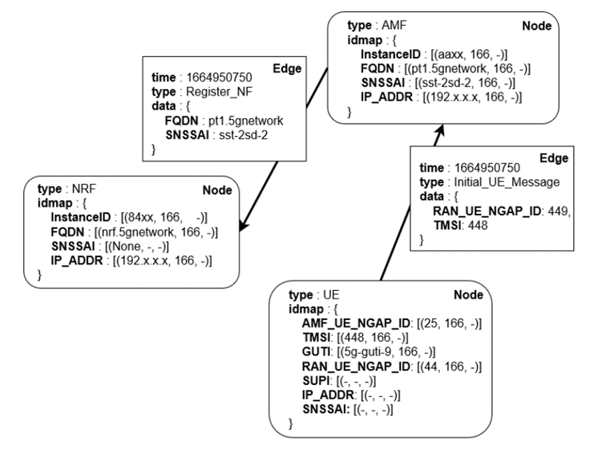
\includegraphics[width=0.7\linewidth]{figures/chapter3/prov5GC.png}
\caption{Trafic de contrôle 5G formalisé par Prov5GC \cite{prov5G} en tant que graphe de provenance}
\label{fig:prov5GCs}
\end{figure}

% Prov5G
Prov5GCC \cite{prov5G} propose de son côté de représenter le trafic sous forme de graphe de provenance. Dans cette représentation, illsutrée sur la figure \ref{fig:prov5GCs}, les nœuds correspondent aux entités du réseau et chaque message échangé entre ces entités est modélisé par une arête, à laquelle est associé le contenu du paquet. La formalisation en graph est particulièrement adaptée à l’analyse topologique des interactions du réseau. Cependant, elle ne modélise pas explicitement la dimension temporelle des échanges, ce qui restreint la capacité à capturer l’évolution dynamique des interactions. De plus, le fait d’agréger le payload au niveau des arêtes limite fortement l’exploitation de l’information contenue dans les paquets. Dans leur cas la payload est utilisé par un algorithme de détection heurisitique spécifique à chaque attaque, ce qui rend l’approche relativement lourde et peu adaptée à des environnements complexes.

\begin{figure}[h]
\centering
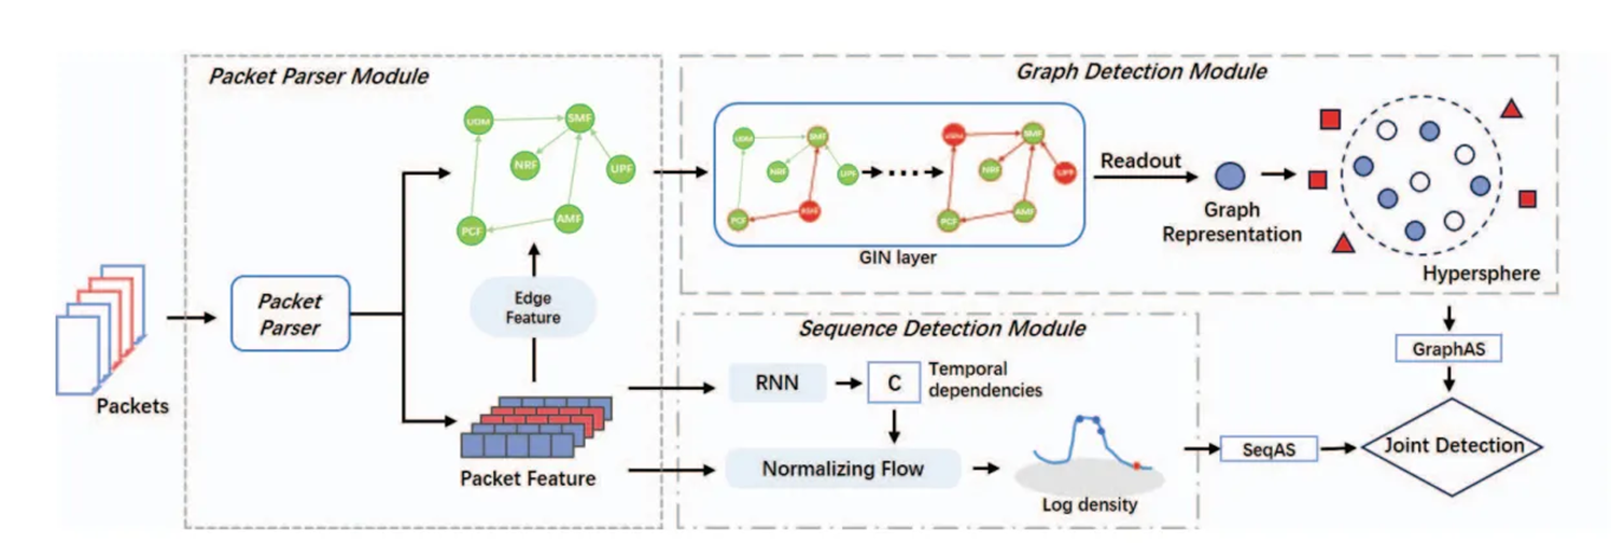
\includegraphics[width=\linewidth]{figures/chapter3/GSAD.png}
\caption{Pipeline de GSAD \cite{gsad} représentant leur formalisation ainsi que les trois modules de détections traitant respectivement les dimensions sémantique, séquentielle et topologique}
\label{fig:gsad}
\end{figure}


% GSAD
GSAD \cite{gsad} propose également de formaliser les données sous forme de graphe, de manière similaire à Prov5GC \cite{prov5G}. La principale différence réside dans la représentation du contenu des arêtes. Au lieu de l’encoder sous forme de dictionnaire monolithique, les auteurs le transforment en flux d’octets structuré comme une image. Cette représentation leur permet d’utiliser un CNN pour encoder chaque paquet et analyser sa dimension sémantique. Les représentations sémantiques sont ensuite injectées dans un GNN afin de modéliser les interactions entre les paquets, puis dans un RNN pour capturer les dépendances temporelles. À notre connaissance, GSAD \cite{gsad} est la seule approche de détection d’anomalies 5G basée sur l’apprentissage profond qui considère simultanément les trois dimensions de détection. La principale limite de leur approche réside dans le fait que, comme évoqué précédemment, les CNN ne permettent qu’une analyse relativement superficielle de la dimension sémantique des paquets. La Figure~\ref{fig:gsad} illustre l’architecture générale du pipeline proposé par GSAD et met en évidence les trois composantes du modèle correspondant respectivement aux trois dimensions.


\begin{table}[h]
\centering
\begin{tabular}{lccc}
\hline
\textbf{Référence} & \textbf{Sémantique} & \textbf{Séquentiel} & \textbf{Topologique} \\
\hline
Kale et al. \cite{ensemble}         & Oui      & Non      & Non \\
Lam et al. \cite{cnn}               & Oui      & Oui      & Non \\
AutoGuard \cite{autoguard}          & Non      & Oui      & Partiel \\
ADSeq-5GCN \cite{adseq}             & Non      & Oui      & Partiel \\
5GCGuard \cite{5GCGuard}            & Non      & Oui      & Partiel \\
Prov5GC \cite{prov5G}               & Partiel  & Non      & Partiel \\
GSAD \cite{gsad}                    & Partiel  & Partiel  & Oui \\
\hline
\end{tabular}
\caption{Comparaison des approches de l'état de l'art de détection d'anomalies 5G selon les dimensions considérées}
\label{tab:sota_comparison}
\end{table}

% Conclusion 
Le tableau \ref{tab:sota_comparison} résume les différentes approches de détection d’anomalies dans les réseaux 5G, en mettant en évidence les dimensions sémantique, temporelle et topologique prises en compte par chacune d’elles. L’état de l’art montre que peu d’approches considèrent simultanément les trois dimensions. Les approches basées sur les GNN apparaissent particulièrement adaptées pour modéliser les interactions entre entités. À l’inverse, aucune des modélisations proposées ne semble réellement adaptée au traitement du contenu sémantique des paquets, celui-ci étant le plus souvent considéré comme un bloc monolithique. Dans ce contexte, nous proposons de représenter le contenu des paquets de manière plus fine en décomposant leurs paramètres en nœuds indépendants. 

\subsection{Comparaison aux techniques utilitées dans les systèmes distribués}
La 5G partage de nombreuses caractéristiques architecturales avec les systèmes distribués modernes. Lorsque l’on s’intéresse à la littérature portant sur la détection d’anomalies dans ce domaine\cite{dist_gnn2}, on constate que les approches proposées reposent principalement soit sur le Federated Learning (FL), afin d’exploiter la nature distribuée des infrastructures, soit sur l’analyse de logs systèmes.

Les approches basées sur le FL, telles que DioT\cite{diot} ou VFL\cite{vfl}, mettent particulièrement en avant les avantages de la fédération pour les systèmes distribués, notamment en matière de passage à l’échelle, de confidentialité et de décentralisation de l’apprentissage. Cependant, leur contribution porte principalement sur le mécanisme de fédération lui-même. Les modèles utilisés restent relativement classiques et ne considèrent généralement qu’une partie des dimensions nécessaires à une détection complète des anomalies. DioT\cite{diot} s’appuie par exemple sur des GRU pour modéliser les dépendances temporelles, tandis que VFL\cite{vfl} exploite GraphSAGE afin de capturer les relations structurelles entre entités.

Les approches basées sur les logs telles que \cite{dist_log1,dist_log2} qui sont très utilisées dans les systèmes distribués présentent également plusieurs limitations. Bien qu’elles permettent d’observer l’activité du système à un haut niveau, les logs constituent une représentation indirecte et partielle des événements réseau. Ils dépendent fortement des implémentations logicielles et peuvent contenir du bruit, des informations manquantes ou des incohérences. Certains événements ou comportements anormaux peuvent ainsi ne jamais être journalisés, limitant la capacité de détection.

Enfin, un grand nombre de travaux restants s’appuient sur des GNN \cite{dist_gnn1,dist_gnn2}, ce qui confirme que la formalisation en graphe est particulièrement adaptée à la modélisation des interactions au sein des systèmes distribués.

\section{Méthodologie de formalisation}
Nous avons vu que le formalisme de graphe était particulièrement adapté à la modélisation de notre problème et qu’il permettait d’intégrer simultanément les dimensions sémantique, temporelle et topologique, comme l’a notamment montré GSAD. La principale différence avec leur formalisation est qu'au lieu de représenter le contenu des paquets comme un bloc monolithique associé à une arête, nous proposons de le décomposer en nœuds indépendants. Nous détaillons à présent notre méthodologie de formalisation. Nous commencerons par l’extraction des caractéristiques à partir du trafic de contrôle, puis nous présenterons leur transformation en graphes adaptés à une analyse par GNN.

\subsection{Extraction des features depuis la payload applicative}
Comme notre objectif est principalement d’analyser le contenu applicatif des paquets, nous extrayons la payload ainsi que l’ensemble des champs disponibles pour chaque paquet. Les seules informations non applicatives conservées concernent la couche IP, utilisées comme identifiant afin de discriminer les différentes entités du réseau. Cette approche n’est pas idéale, car elle est sensible au \textit{spoofing}. Toutefois, dans un cadre opérationnel, ces identifiants pourraient être remplacés par des mécanismes plus robustes, tels que des empreintes ou des hash représentant les entités de manière unique.

Pour récupérer le contenu des payloads, nous utilisons \textit{Scapy}, qui permet de parser les paquets réseau et de générer, pour chacun d’eux, une représentation sous forme de dictionnaire associant les champs à leurs valeurs respectives.

Un des problèmes rencontrés concerne certains paquets, notamment HTTP/2, qui contiennent principalement des structures JSON fortement imbriquées, ce qui introduit une complexité supplémentaire. La conservation explicite du chemin d’imbrication dans notre formalisme modifierait fortement la structure du graphe et accorderait une importance excessive à cette information. L’imbrication est utile pour différencier des paramètres, mais reste secondaire par rapport aux valeurs elles-mêmes.

Pour gérer ce problème, nous avons donc choisi d’aplatir les dictionnaires extraits des payloads en construisant le nom de chaque paramètre de feuille comme la concaténation de ses clés le précédantes, séparées par des délimiteurs. On obtient ainsi des identifiants de paramètres composés, par exemple \texttt{http2.headers.content-type}, permettant de désigner le champ \texttt{content-type} d’un paquet HTTP/2. Cette approche permet de conserver l’information d’imbrication tout en maintenant une structure suffisamment simple pour notre formalisation en graphe.

\subsection{Transformation en graph}

\begin{figure}[h]
\centering
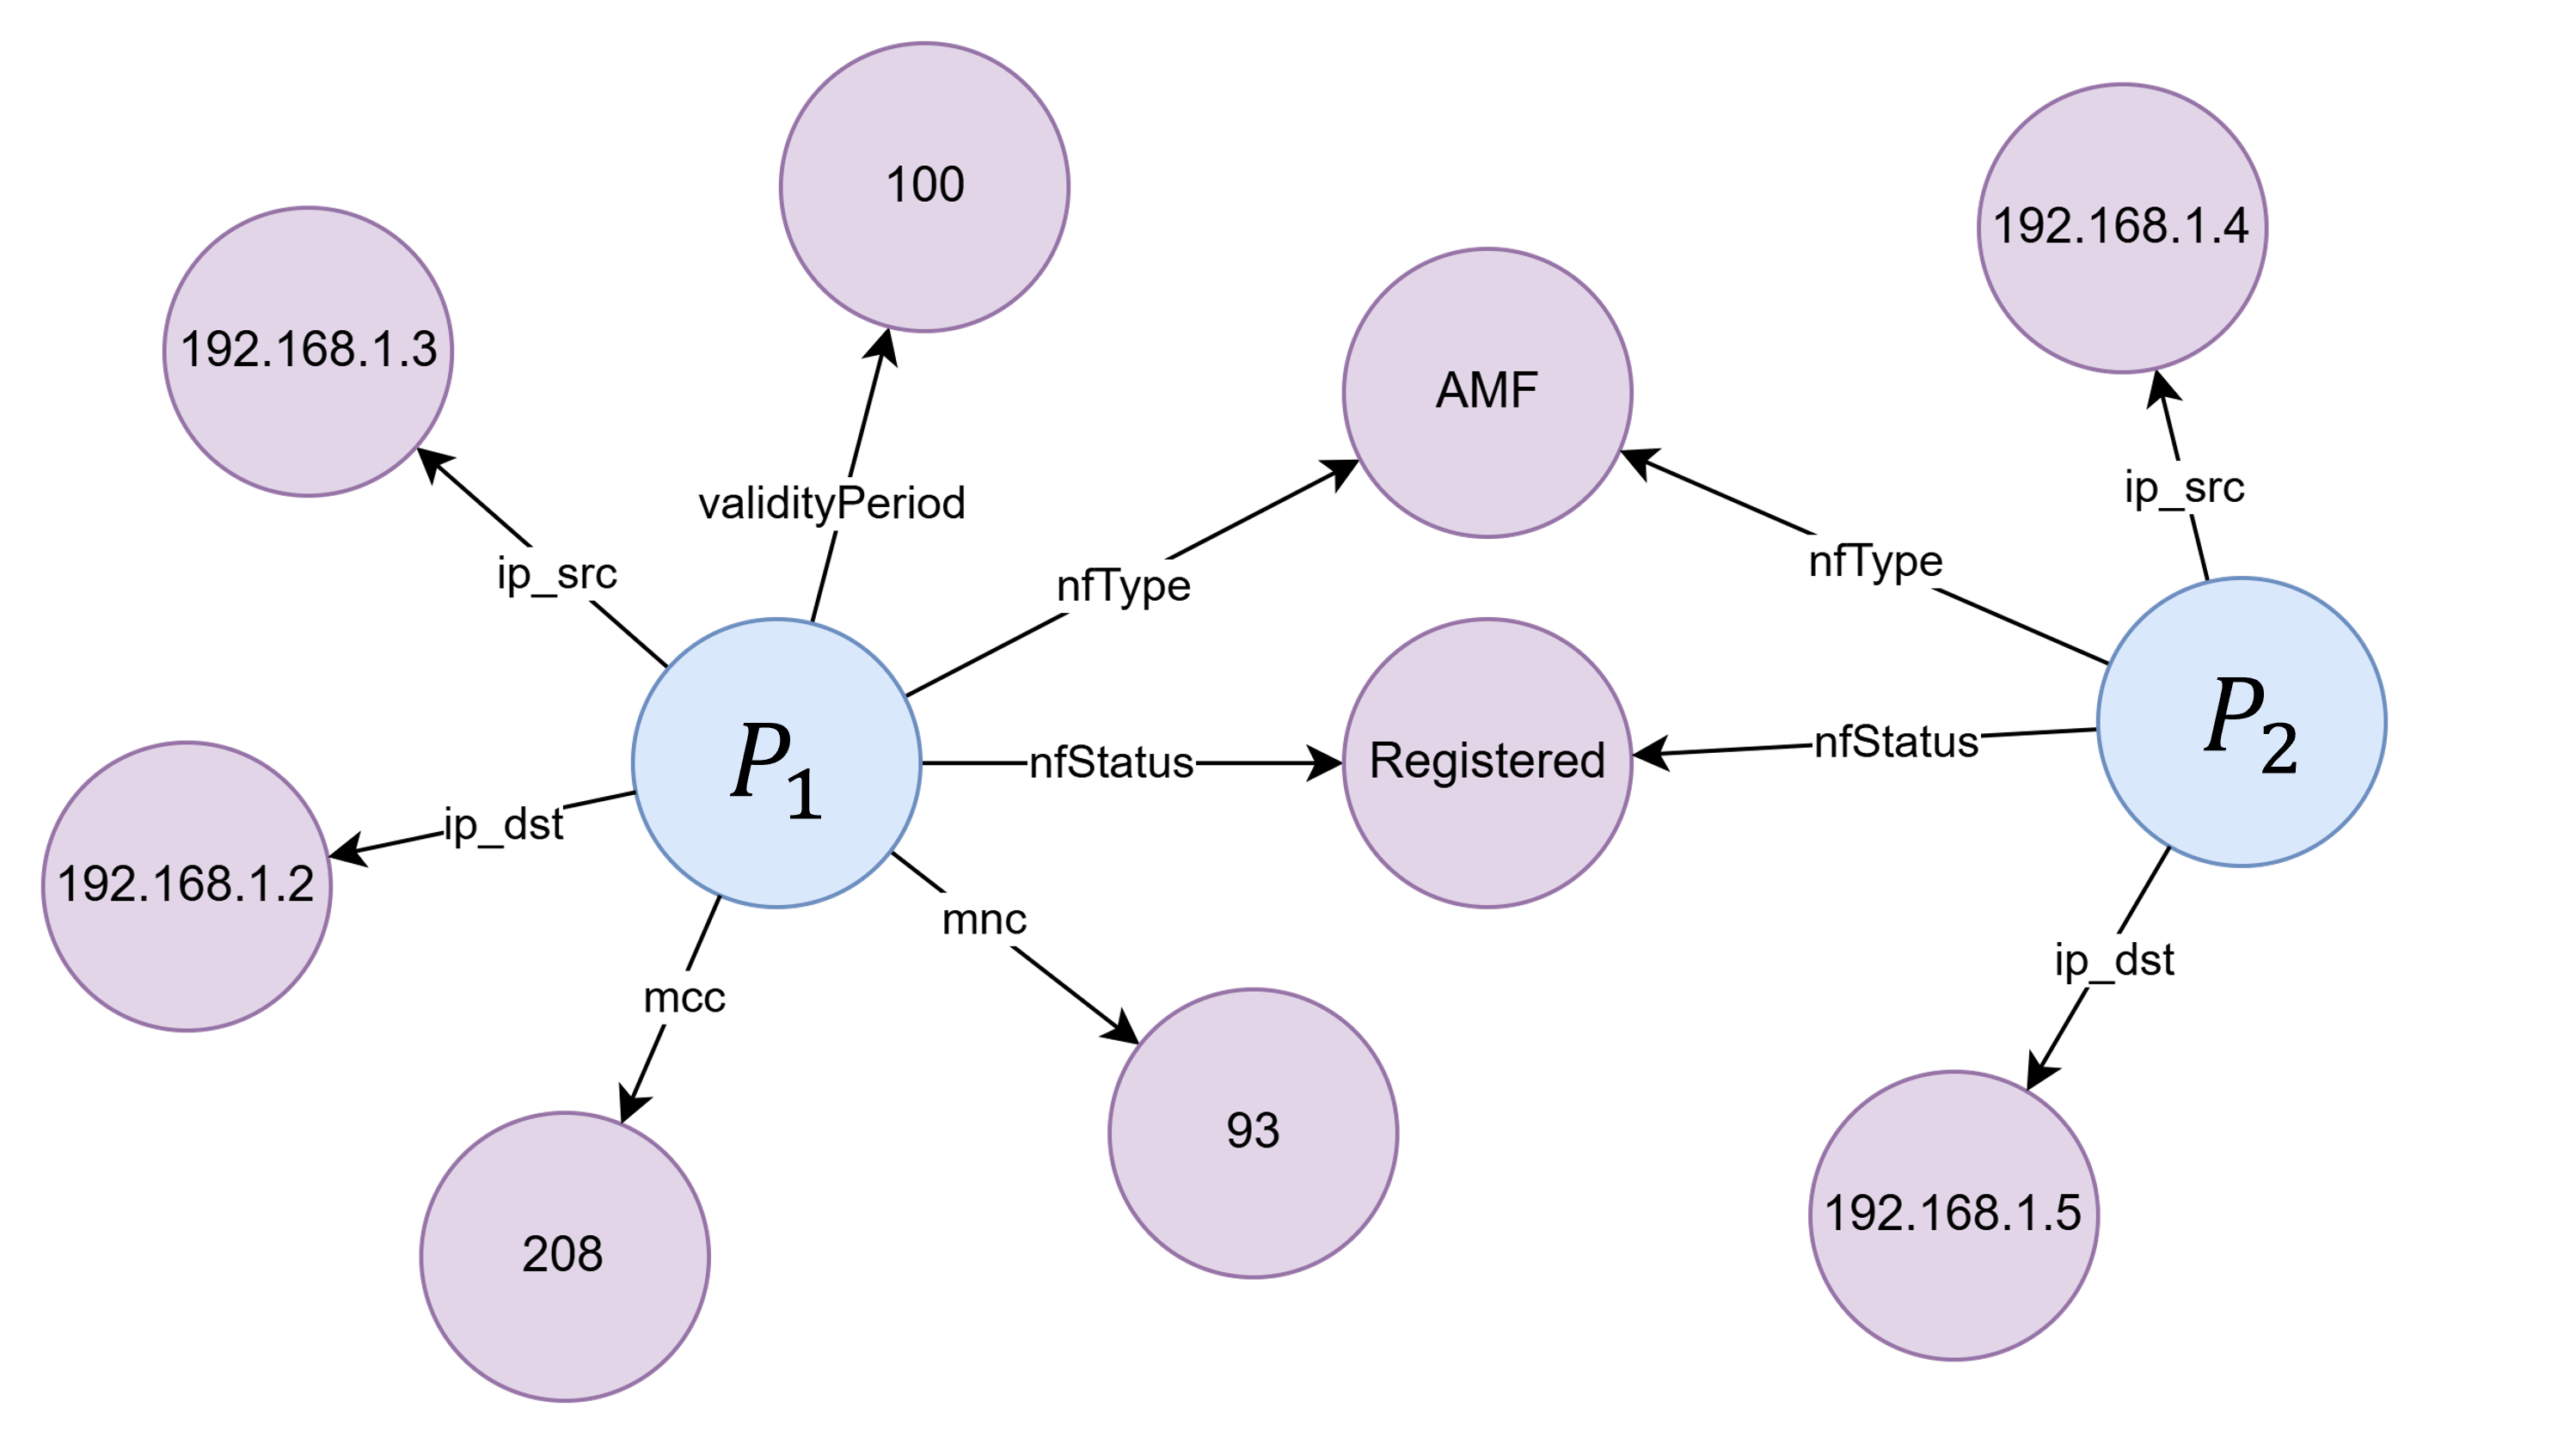
\includegraphics[width=0.7\linewidth]{figures/chapter3/graph_example.png}
\caption{Exemple de transformation de paquets en sous-graphes. Les nœuds mauves représentent les valeurs des paramètres, tandis que les nœuds bleus représentent les paquets eux-mêmes.}
\label{fig:graph_example}
\end{figure}

À la réception d’un paquet, au lieu de le représenter comme une arête entre deux entités, nous le modélisons sous forme de sous-graphe, où chaque paramètre est encodé comme un nœud indépendant relié à un nœud central qui représente le paquet. Chaque nœud de feature contient la valeur du champ associé, tandis que l’arête reliant ce nœud au paquet porte le nom du paramètre correspondant. À chaque nouveau paquet observé, un sous-graphe est créé. Pour chaque paramètre, un nouveau nœud est ajouté s’il n’a pas encore été rencontré. Dans le cas contraire, le nœud existant est réutilisé. Ce mécanisme permet de relier progressivement les différents sous-graphes entre eux à travers les paramètres partagés. La figure \ref{fig:graph_example} illustre le processus de transformation de deux paquets en deux sous graphes. Ces deux paquets partagent certains paramètres ayant des valeurs communes et leurs sous-graphes respectifs se retrouvent donc connectés. Comme il n’existe pas d’arcs reliant des nœuds de type paramètre entre eux, ni de nœuds centraux entre eux, on obtient ainsi un graphe biparti. Une autre caractéristique de notre graphe est qu’il est purement additif : la réception d’un paquet ne peut entraîner que l’ajout de nouveaux nœuds et d’arêtes, sans jamais modifier ni supprimer ceux déjà présents.

Cette décomposition permet de connecter des attributs issus de paquets différents en s’appuyant sur des caractéristiques communes, plutôt que sur la seule structure source–destination. Une telle représentation offre un niveau de granularité très fin et permet de capturer des interactions plus riches entre les caractéristiques des paquets. De plus, cette approche permet également d’identifier précisément les paramètres à l’origine d’un comportement anormal et se révèle donc, par construction, hautement interprétable.

Nous allons maintenant voir à quoi ressemblent les anomalies de chaque dimension une fois transformées en graphe.

\subsubsection{Anomalies sémantiques}

\begin{figure}[h]
\centering
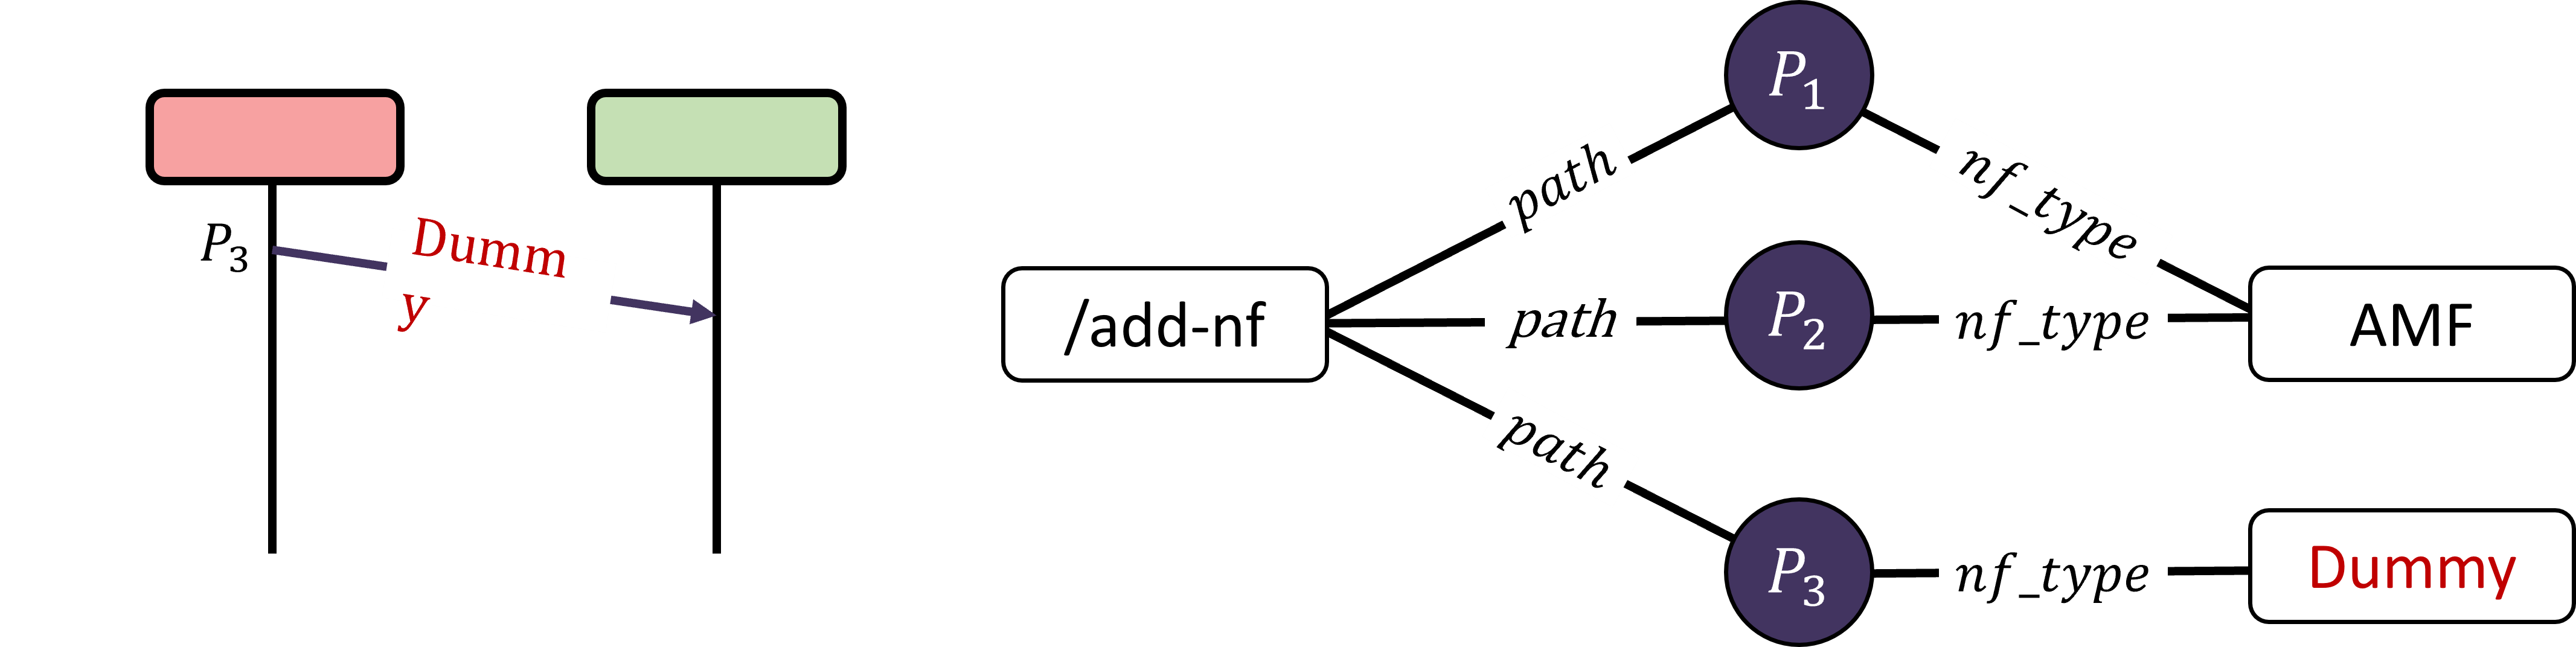
\includegraphics[width=\linewidth]{figures/chapter3/graph_semantique.png}
\caption{Anomalie sémantique et sa représentation sous forme de graphe}
\label{fig:graph_semantic}
\end{figure}

La figure \ref{fig:graph_semantic} illustre une anomalie sémantique dans laquelle un champ inhabituel apparaît. Dans le cas présent, il s’agit du paquet P3 qui contient la valeur \textit{NF Type} qui n'existe pas en 5G. Cette anomalie peut être détectée en le comparant aux autres paquets de même nature. On observe par exemple que les paquets P1 et P2, qui sont, comme P3, des requêtes vers l’endpoint \textit{add-nf}, possèdent des valeurs identiques pour le champ \textit{nf-type}, alors que P3 s’en écarte. Un modèle de détection ayant appris la structure usuelle de ce type de paquet pourrait ainsi identifier l’anomalie en observant uniquement le sous-graphe associé à P3.

\subsubsection{Anomalies topologiques}

\begin{figure}[h]
\centering
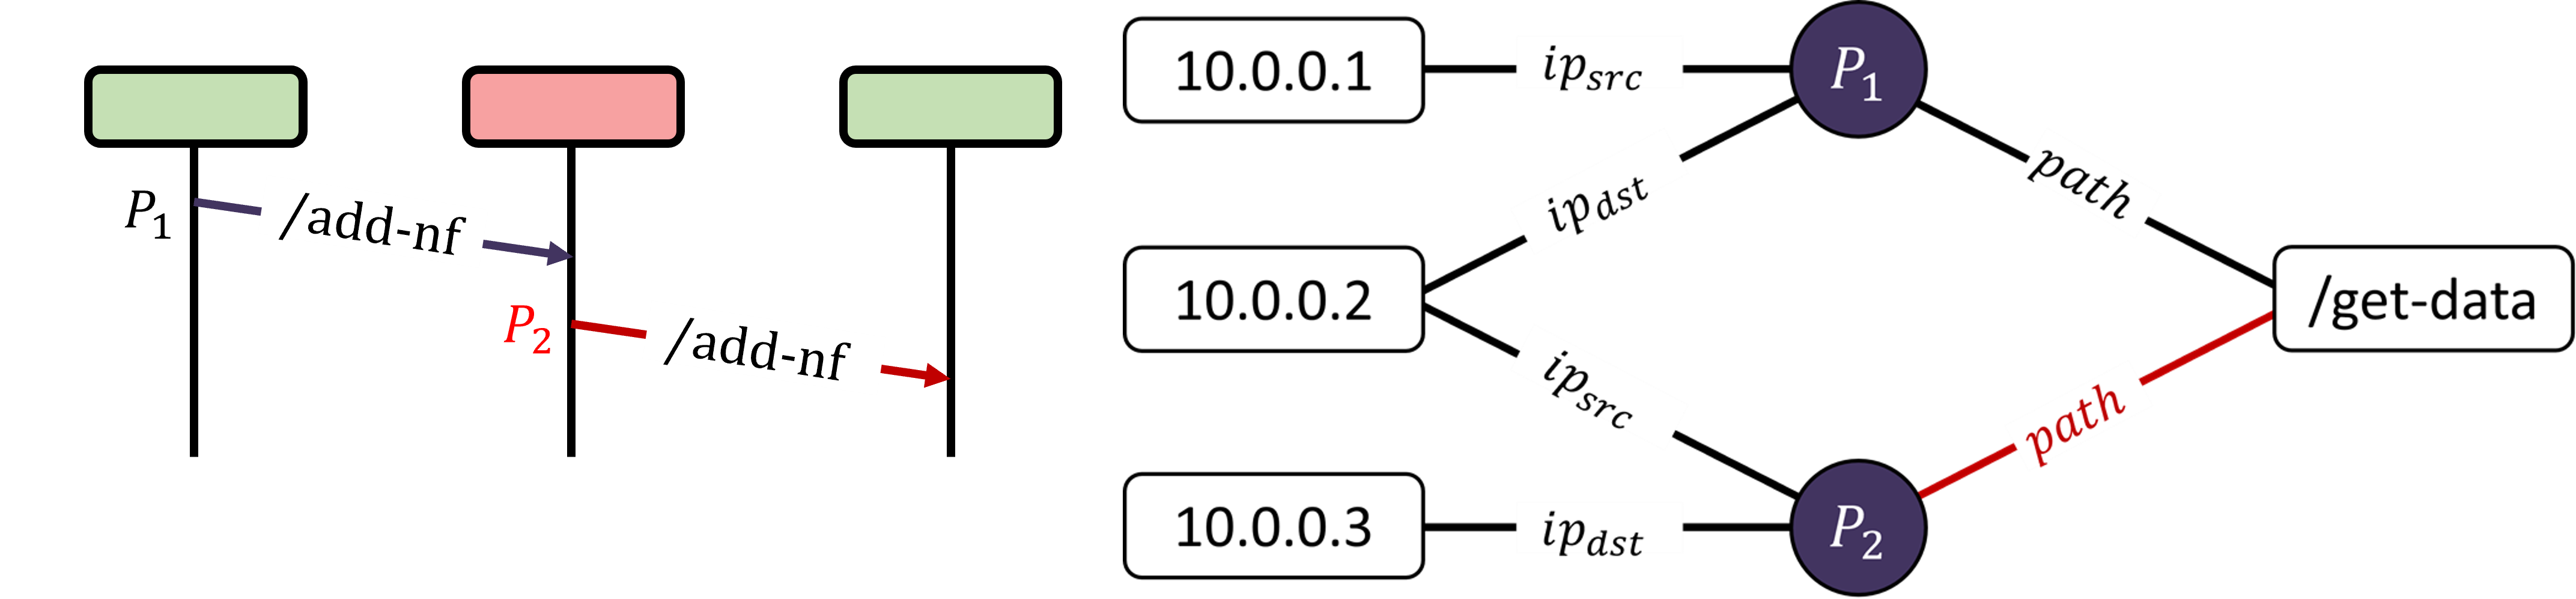
\includegraphics[width=\linewidth]{figures/chapter3/graph_topologique.png}
\caption{Anomalie topologique et sa représentation sous forme de graphe}
\label{fig:graph_topological}
\end{figure}

Sur la figure \ref{fig:graph_topological}, on observe un exemple d’attaque de type man-in-the-middle, où un paquet P1, initialement envoyé à l’adresse \textit{10.0.0.2}, génère l’envoi d’un nouveau paquet P2 identique (ici simplifié par le fait qu’il s’agisse du même endpoint), avec comme source la destination du paquet précédent et comme destination une nouvelle adresse. Ce cas ne peut normalement pas survenir en 5G, car il n’existe aucun scénario légitime de redirection de trafic de ce type. Le paquet P2 est une copie de P1 et paraît donc légitime pris individuellement. Il est nécessaire de prendre en compte le contexte de redirection afin de détecter l’anomalie.

\subsubsection{Anomalies séquentielles}

\begin{figure}[h]
\centering
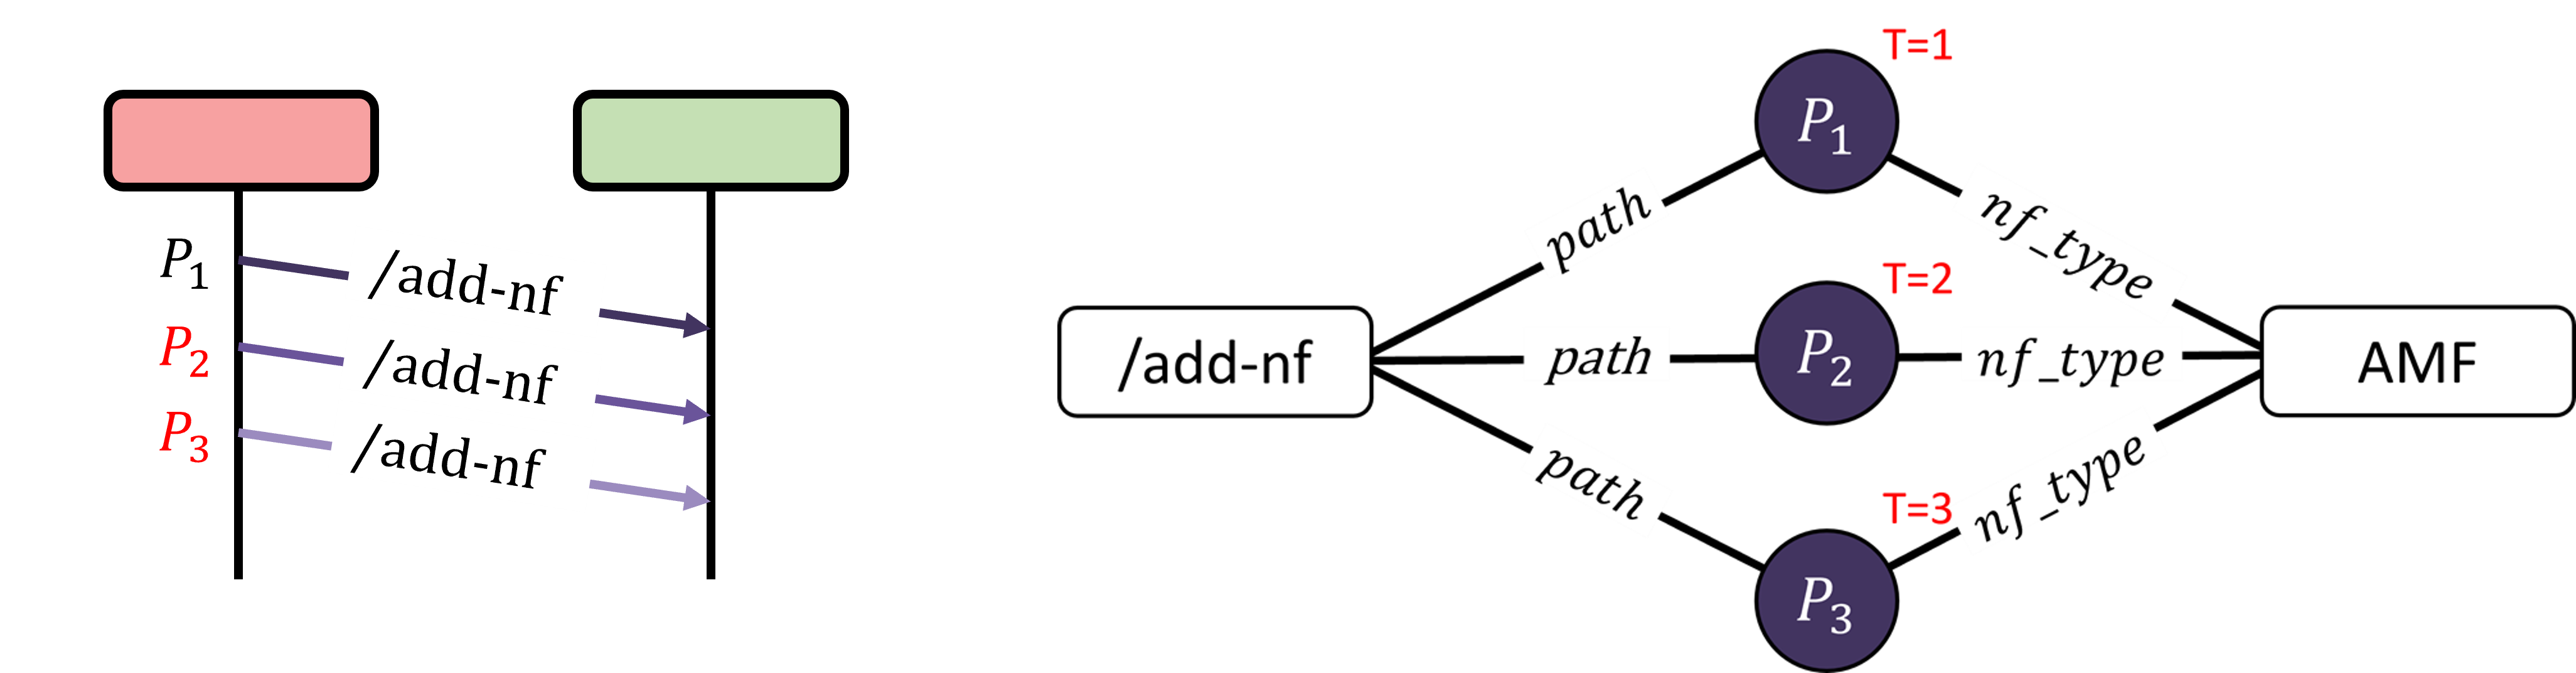
\includegraphics[width=\linewidth]{figures/chapter3/graph_seq.png}
\caption{Anomalie séquentielle et sa représentation sous forme de graphe}
\label{fig:graph_sequential}
\end{figure}

Enfin, sur la figure \ref{fig:graph_sequential}, on observe un exemple d’anomalie séquentielle. Dans ce cas, le contenu et les interactions des paquets sont normaux et la caractéristique anormale concerne uniquement leur ordre d'arrivée. Le problème est que le formalisme actuel ne modélise pas explicitement la dimension temporelle. Il serait possible de l’intégrer en ajoutant à chaque sous-graphe un nœud représentant le temps d’observation du paquet, mais avec cette approche la dimension temporelle serait confondue avec les autres paramètres, alors qu’elle est de nature distincte et particulièrement importante. Il est donc nécessaire de proposer une modélisation permettant d’intégrer le temps de manière plus explicite. Pour cela, nous nous intéressons aux graphes dynamiques, qui intègrent nativement la dimension temporelle, et que nous présentons dans les sections suivantes.

\section{Détection d’anomalies dans des graphs}

\subsection{Introduction aux GNN}

\begin{figure}[h]
\centering

\begin{minipage}{0.32\linewidth}
    \centering
    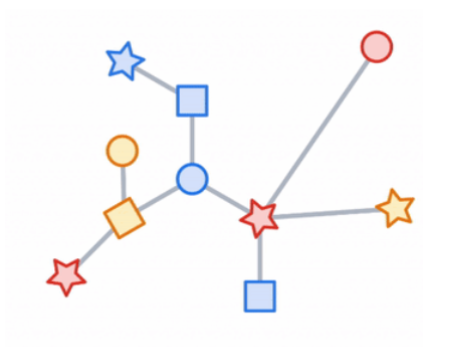
\includegraphics[width=\linewidth]{figures/chapter3/conv_1.png}
\end{minipage}
\hfill
\begin{minipage}{0.32\linewidth}
    \centering
    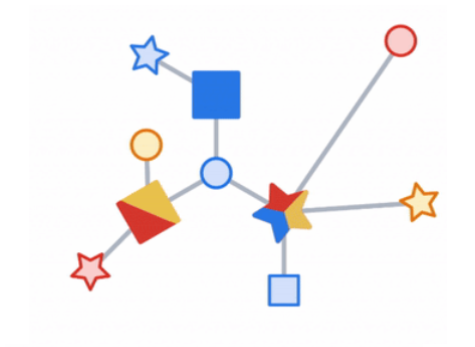
\includegraphics[width=\linewidth]{figures/chapter3/conv_2.png}
\end{minipage}
\hfill
\begin{minipage}{0.32\linewidth}
    \centering
    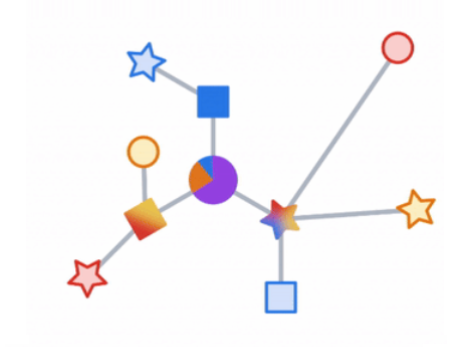
\includegraphics[width=\linewidth]{figures/chapter3/conv_3.png}
\end{minipage}

\caption{Illustration du processus de convolution. La première figure représente le graphe à son état initial. Dans la deuxième, une convolution est appliquée : on observe que les informations des nœuds feuilles sont agrégées et propagées à leurs voisins directs. Dans la troisième, une deuxième convolution est réalisée, et les informations précédemment propagées sont à nouveau diffusées jusqu’au nœud central du graphe, qui contient ainsi une représentation de son voisinage complet à distance 2.}
\label{fig:convolution}
\end{figure}

De manière générale, les graph neural networks sont très proches des CNN présentés précédemment. La principale différence est que les CNN opèrent sur des images, tandis que les GNN travaillent directement sur des graphes. Dans les deux cas, le principe repose sur une agrégation locale de l’information. Dans une image, cette agrégation s’effectue sur des voisinages de pixels, tandis que dans un graphe elle s’applique au voisinage des nœuds. Certains travaux proposent notamment de considérer une image comme un graphe de pixels et d’y appliquer des GNN, mais il s’agit d’une approche relativement marginale \cite{gnn_image}. L’idée fondamentale de ces deux types de modèles est que chaque itération du processus de convolution permet de diffuser l’information aux voisins directs. En procédant de manière récursive, chaque couche de convolution propage cette information à une distance croissante, augmentant progressivement le champ de réception des représentations. La figure \ref{fig:convolution} illustre ce processus de diffusion de l’information à travers réalisé par deux convolutions successives.

\subsection{Etat de l'art des GNN}
Le domaine des GNN est relativement récent et s’est fortement développé au cours de la dernière décennie. Le concept de réseaux de neurones sur graphes a été formellement introduit pour la première fois en 2008 par Scarselli et al.~\cite{gnn}, qui ont proposé un cadre neuronal pour l’apprentissage sur des données structurées en graphe, basé sur des mécanismes itératifs de propagation et d’agrégation d’états. Des travaux ultérieurs ont considérablement amélioré la praticabilité et la scalabilité de cette formulation initiale. En particulier, Kipf et Welling~\cite{gcn} ont introduit les Graph Convolutional Networks (GCN), qui simplifient le processus de propagation des messages en linéarisant l’agrégation de voisinage.

Dans leur formulation moderne, les GNN peuvent être vus comme réalisant des convolutions basées sur le voisinage, où l’information provenant des nœuds adjacents est agrégée afin d’enrichir la représentation de chaque nœud avec un contexte local. La plupart des architectures contemporaines de GNN suivent le paradigme de \textit{message passing} proposé par Gilmer et al.~\cite{mpnn}, composé de trois phases principales : la construction des messages à partir des embeddings des nœuds, l’agrégation des messages provenant des voisins, et la propagation (ou mise à jour) de l’information agrégée pour produire de nouvelles représentations des nœuds.

Sur la base du cadre MPNN standard, plusieurs extensions ont été proposées. Par exemple, les Graph Attention Networks (GAT)~\cite{gat} introduisent des mécanismes d’attention qui attribuent des poids adaptatifs aux nœuds voisins lors de l’agrégation. GraphSAGE~\cite{graphsage} permet un apprentissage inductif sur des nœuds jusqu’alors non vus en échantillonnant un voisinage de taille fixe et en appliquant des fonctions d’agrégation apprenables telles que la moyenne, le pooling ou des agrégateurs basés sur LSTM. D’autres variantes notables incluent les Graph Isomorphism Networks (GIN)~\cite{gin}, qui atteignent un pouvoir discriminant maximal parmi les GNN basés sur l’agrégation de voisinage.

Cependant, la plupart de ces architectures de GNN sont principalement conçues pour des graphes statiques. Or, nos données évoluent dans le temps et le graphe sous-jacent est dynamique. Nous nous intéressons donc aux modèles de graphes dynamiques, une classe encore plus récente de GNN. Parmi ces modèles, on distingue deux grandes catégories selon la granularité temporelle.

La première famille, les réseaux de graphes à temps discret (DTGN), constitue l’approche la plus directe pour intégrer l’information temporelle. Parmi les exemples notables de DTGN figurent EvolveGCN~\cite{evolvegcn} et T-GCN~\cite{tgcn}, qui appliquent des opérations GNN classiques sur des captures de l'état du graphe à intervalle régulier. Dans ce cas, la dimension temporelle est capturée de façon externe à l’aide de modèles récurrents utilisés en complément du GNN.

La seconde catégorie correspond aux réseaux de graphes en temps continu, qui opèrent à une granularité temporelle plus fine que les approches discrètes. Plutôt que de reposer sur des instantanés fixes, ces modèles traitent des séquences d’événements correspondant à l’ajout, la suppression ou la modification de nœuds et d’arêtes dans le graphe. Cette modélisation au niveau événementiel permet d’intégrer directement les dépendances temporelles dans le modèle, plutôt que de les traiter de manière externe. Un exemple emblématique de cette approche est le Temporal Graph Network (TGN)~\cite{tgn}, qui maintient des embeddings de nœuds évolutifs mis à jour en réponse aux événements entrants à l’aide d’une combinaison de mécanismes de message passing et de mémoire.

Une vue d’ensemble de l’apprentissage sur graphes dynamiques est proposée par Feng et al.~\cite{survey_gnn}, qui présentent une synthèse mettant en évidence les différences conceptuelles entre les modèles dynamiques à temps discret et à temps continu, ainsi qu’un benchmark étendu des principales méthodes de ces deux catégories.

\subsection{Formalismation adapté à l'utilisation de GNN dynamiques}
Pour considérer la dimension temporel et détecter les attaques de flood and multi-stage, il faut intégrer l'information temporel à notre détection et donc considérer les graphs dynamiques. On pourrait utiliser les graphs dynamiques discrets et c'est ce que fait d'ailleurs GSAD \cite{gsad}. Cette façon de gérer les graphes dynamiques est facile à comprendre et à implémenter, car les captures à intervalle régulier de l'état du graph forment une séquence de graphs indépendants sur lesquels on peut appliquer les GNN traditionnels sans modification majeure. Leur principal inconvénient est qu'ils sont très lourds et peu efficaces pour détecter les dépendances sur de longues périodes.

\begin{figure}[h]
\centering

% --- Première ligne ---
\begin{subfigure}{0.49\linewidth}
    \centering
    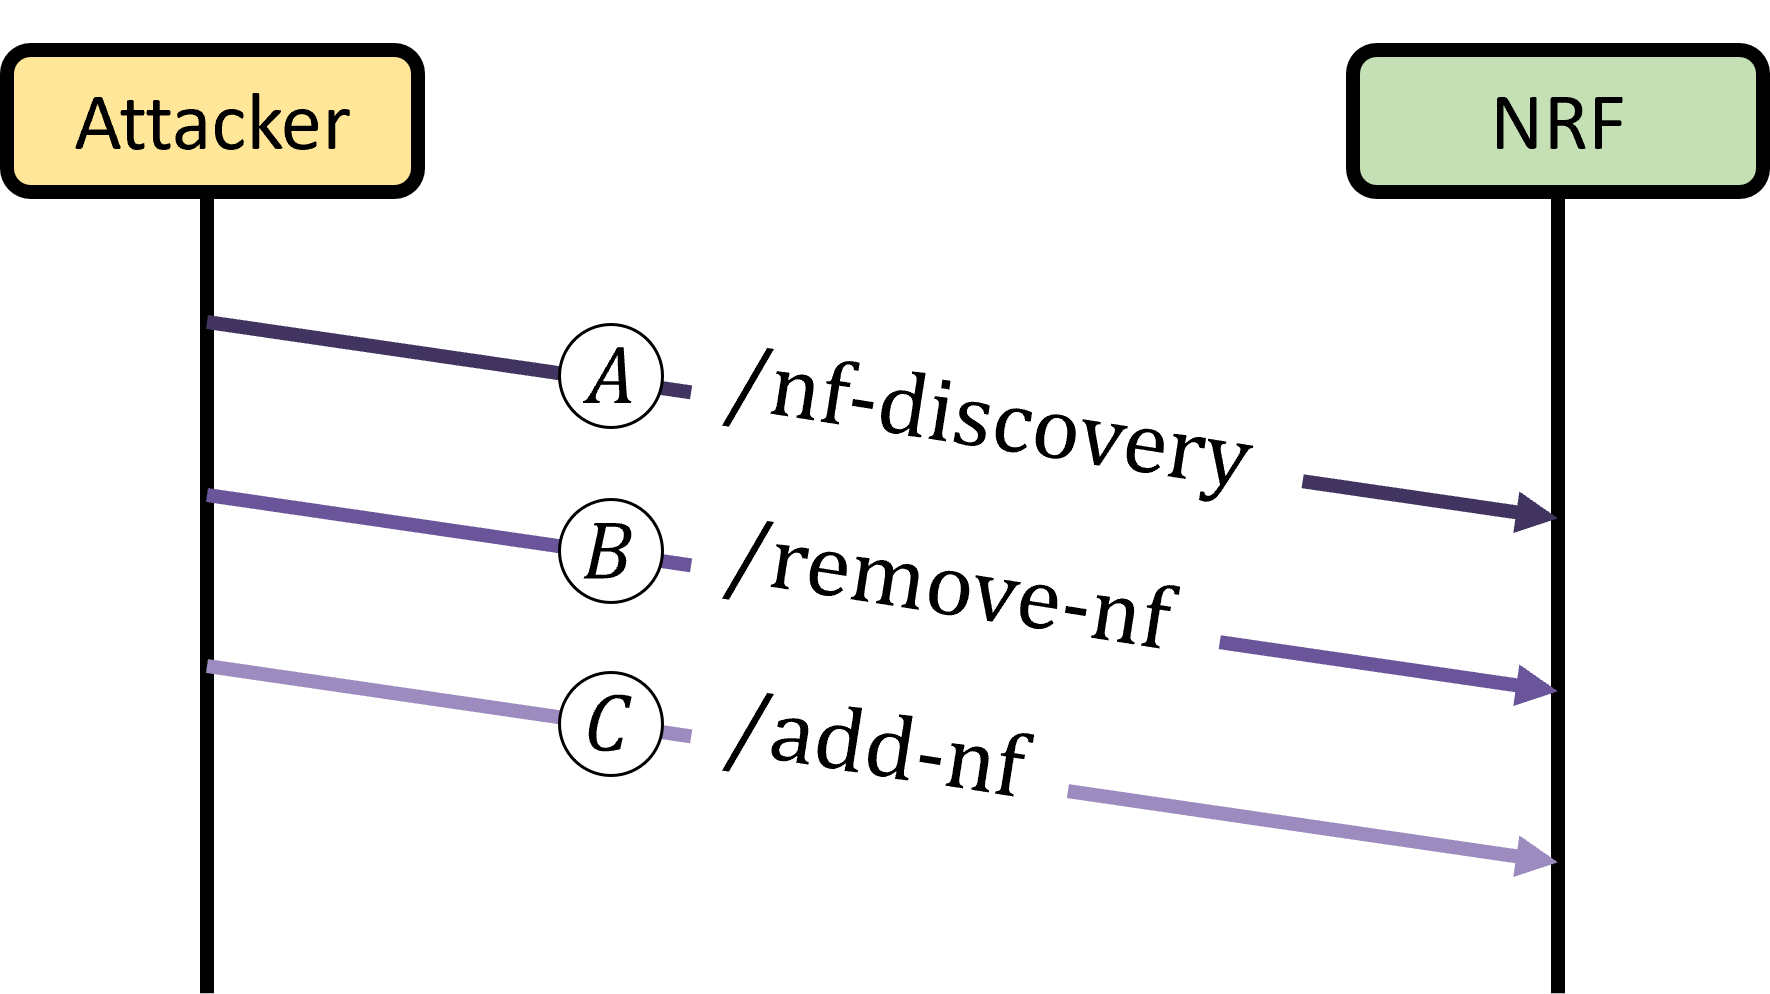
\includegraphics[width=\linewidth]{figures/chapter3/graph_continu_p1.png}
    \caption{Séquence d’envoi de trois paquets vers le NRF à des endpoints distincts.}
\end{subfigure}
\hfill
\begin{subfigure}{0.49\linewidth}
    \centering
    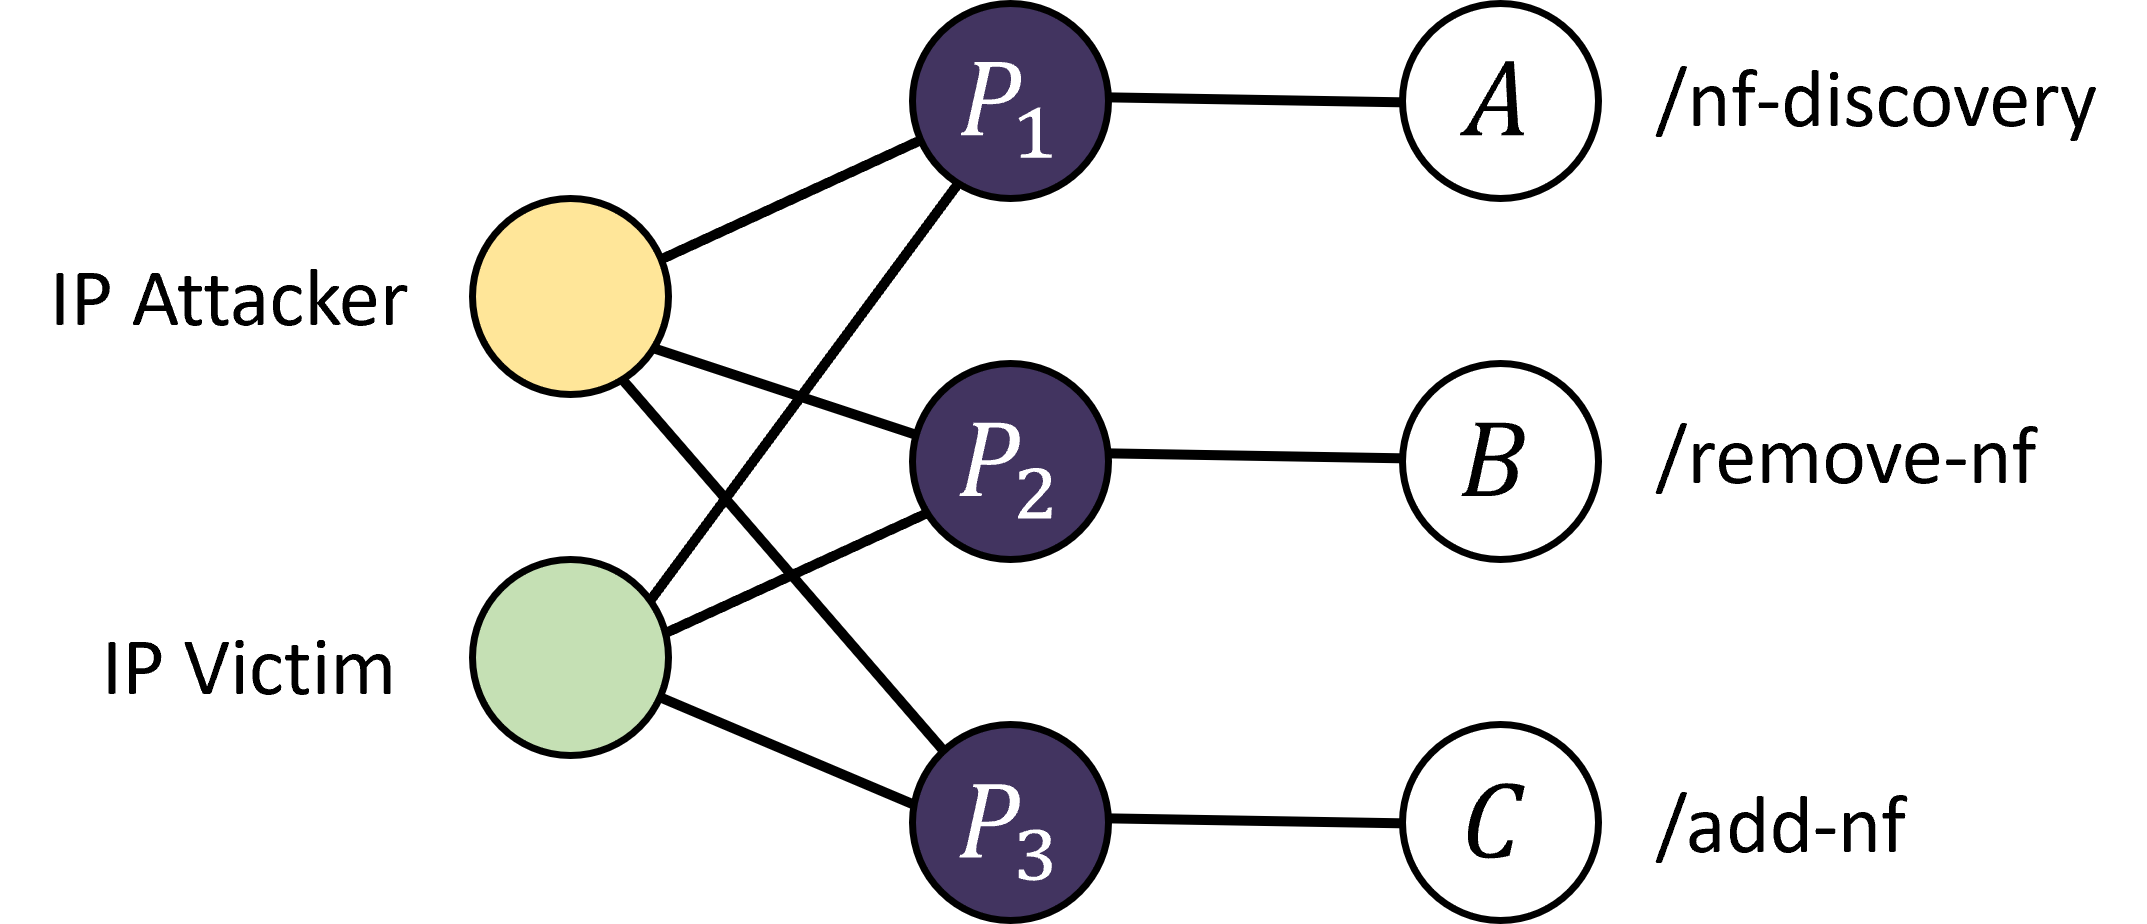
\includegraphics[width=\linewidth]{figures/chapter3/graph_continu_p2.png}
    \caption{Représentation sous forme de graphe statique. Chaque paquet génère un sous-graphe relié par des paramètres communs.}
\end{subfigure}

\vspace{0.5cm}

% --- Deuxième ligne ---
\begin{subfigure}{\linewidth}
    \centering
    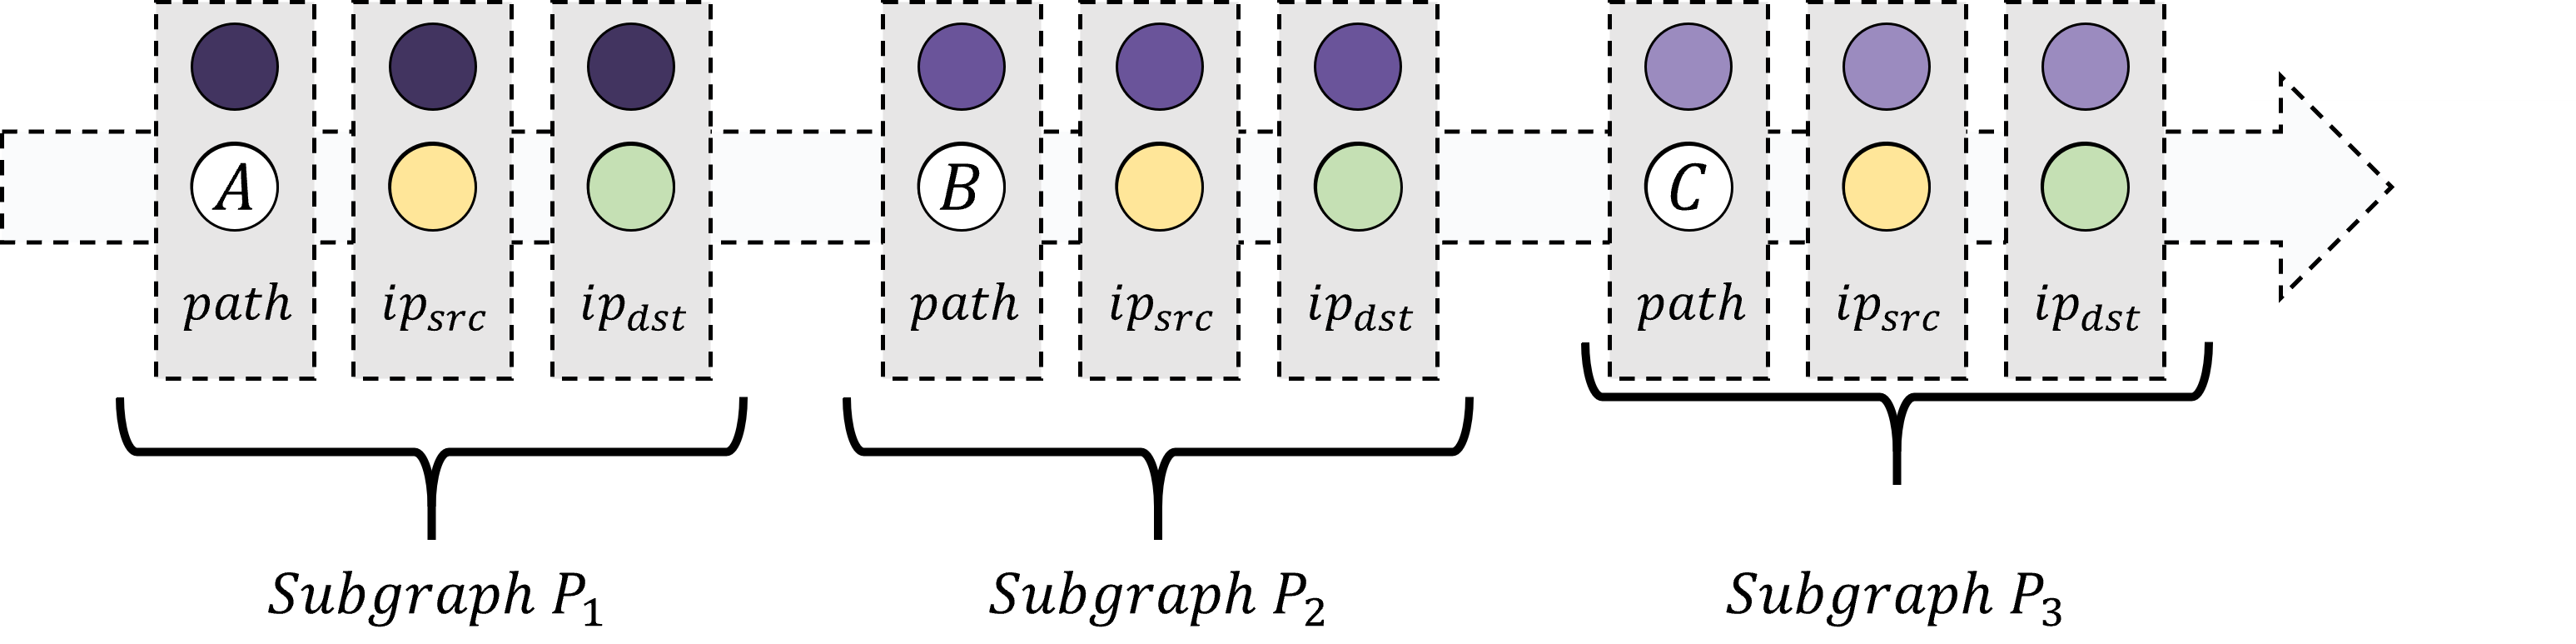
\includegraphics[width=\linewidth]{figures/chapter3/graph_continu_p3.png}
    \caption{Passage vers un graphe dynamique continu, où chaque arête est modélisée comme un événement contenant les informations des nœuds et arcs concernés.}
\end{subfigure}

\caption{Différentes représentations d’une même séquence d’échanges entre un attaquant et le NRF : diagramme de séquence, graphe statique, puis graphe dynamique continu.}
\label{fig:graph_continu}
\end{figure}

Nous nous intéressons donc davantage aux graphes dynamiques continus, tels qu’introduits dans le cadre de TGN~\cite{tgn}. Dans cette approche, plutôt que de représenter le graphe comme un objet statique décrivant un état à un instant donné, celui-ci est modélisé comme une séquence d’événements qui le construit progressivement.

\[
\mathcal{G} = \{ e_1, e_2, \dots, e_n \}
\]
où $e_i$ désigne l’événement apparaissant à la $i$-ème position dans la séquence.

Ces événements correspondent généralement à des ajouts, suppressions ou modifications de nœuds et d’arêtes. Toutefois, notre cadre est plus simple car notre graphe est purement additif. Chaque arête qui serait ajoutée dans un graphe traditionnel est représentée comme un événement défini par cette arête ainsi que par les deux nœuds qu’elle relie. 

\[
e_i = (u, v_i, x_i),
\]
où $u \in \mathcal{V}_c$ désigne un nœud central, $v_i \in \mathcal{V}_f$ un nœud de paramètre contenant la valeur de ce dernier et $\mathbf{z}_i \in \mathbb{R}^d$ le nom du paramètre contenu dans l’arête. 

Cette formulation nécessite d’adapter les algorithmes classiques utilisés dans les GNN, mais elle permet une représentation beaucoup plus fine, dans laquelle aucune information temporelle n’est perdue. La figure \ref{fig:graph_continu} illustre la transformation d'une forme de graphe statique à celle d'un graphe dynamique continu.

\subsection{Fonctionnement détaillé d'un GNN dynamique}
Pour comprendre le fonctionnement d’un GNN dynamique continu, nous allons nous appuyer sur le fonctionnement du Temporal Graph Network (TGN), l’un des modèles les plus populaires de cette catégorie. La plupart des GNN dynamiques suivent en effet une architecture globale très similaire, ce qui fait de TGN un exemple représentatif de la conception générale de cette famille de modèles. La figure \ref{fig:tgn} illustre l’architecture de TGN, qui se compose de quatre modules principaux : un module de mémoire, un module d’agrégation de messages, un module de mise à jour de la mémoire et un module d’inférence.

\begin{figure}[h]
\centering
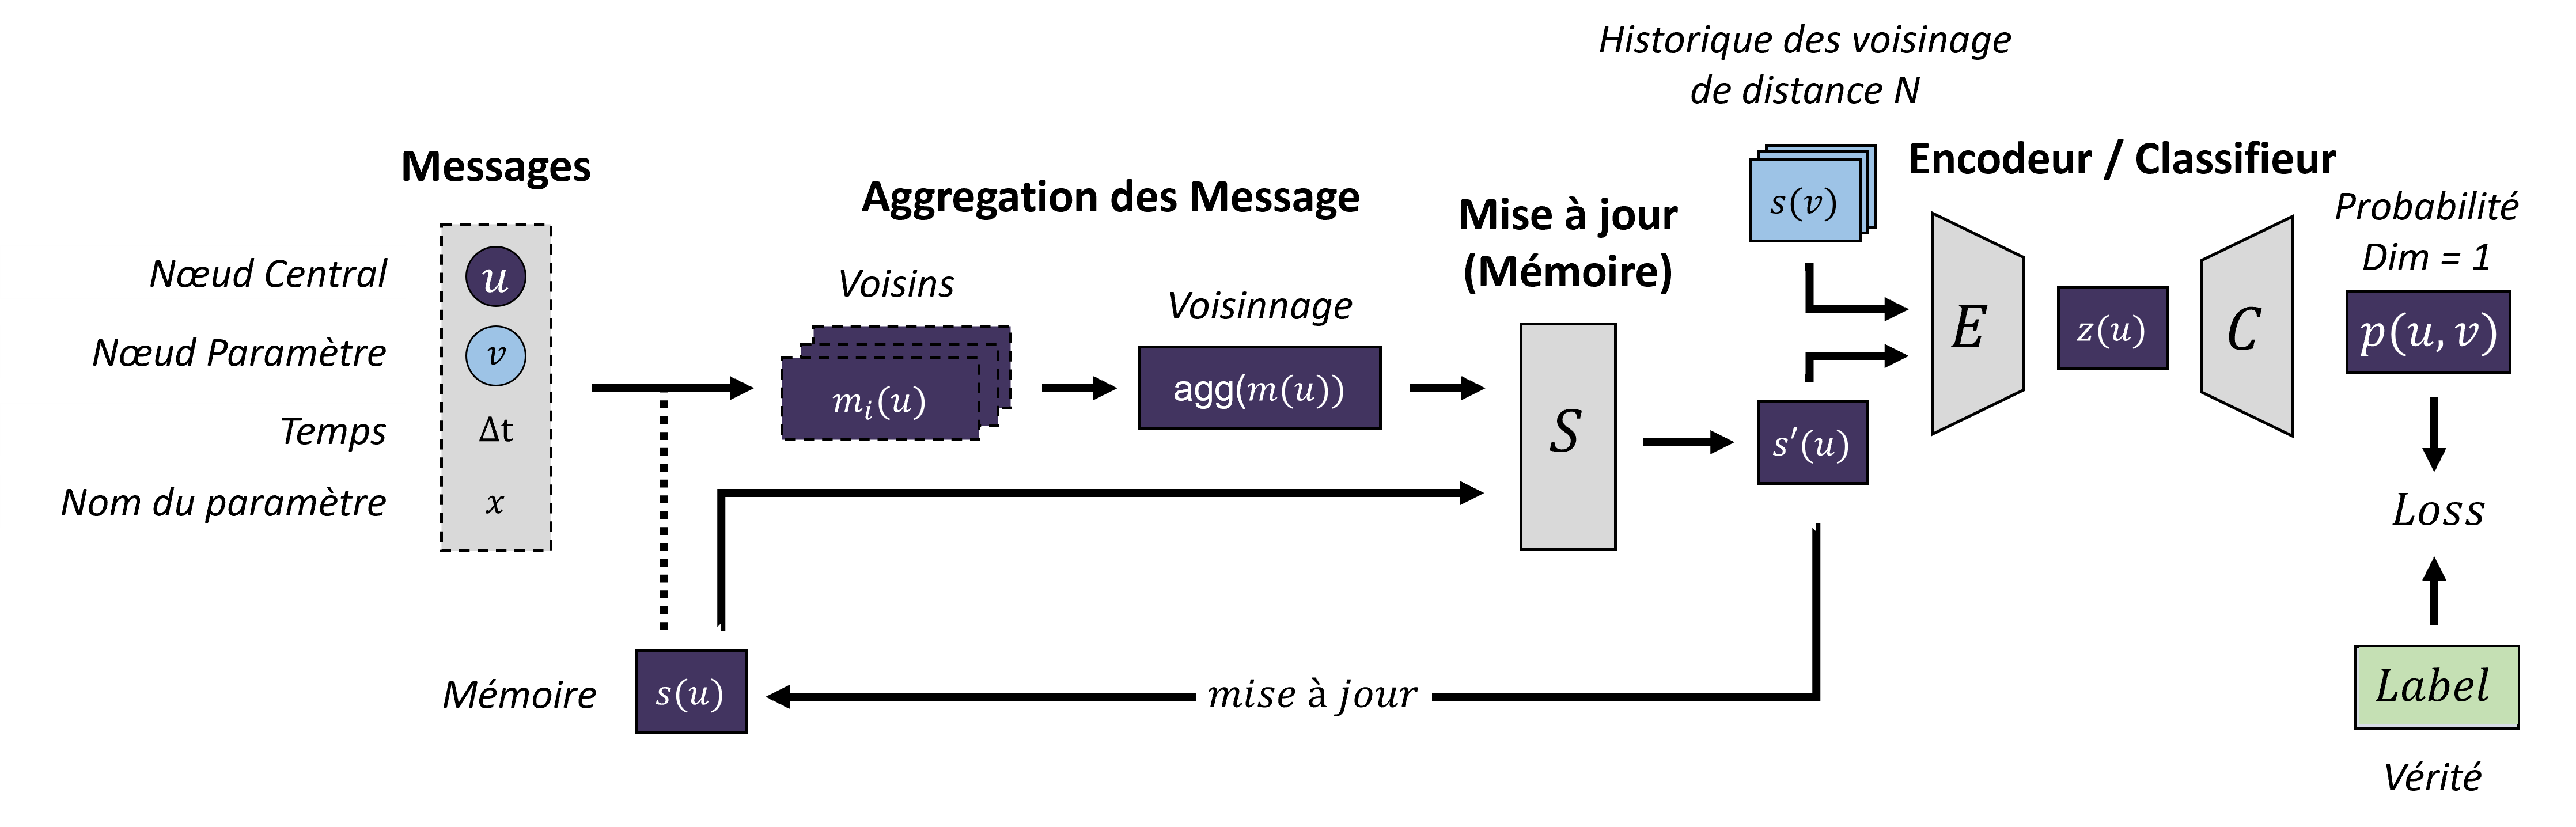
\includegraphics[width=\linewidth]{figures/chapter3/tgn.png}
\caption{Vue d'ensemble de l'architecture de TGN, illustrant les quatre modules principaux : mémoire, agrégation de messages, mise à jour de la mémoire et inférence.}
\label{fig:tgn}
\end{figure}

\subsubsection{Création des messages}
La première étape consiste à construire un message, c’est-à-dire un vecteur contenant l’ensemble des informations encodées associées à un événement du graphe dynamique. Dans un premier temps, les vecteurs associés aux nœuds centraux et aux nœuds paramètres sont initialisés comme des vecteurs nuls. Si ces nœuds ont déjà été impliqués dans des événements précédents, leurs représentations précédemment calculées est alors réutilisées. Le vecteur associé à l’arête est quant à lui déterminé à partir du nom du paramètre porté par l’événement. Dans notre cas, ce nom de paramètre correspond à un token textuel et il est donc nécessaire de l’encoder au préalable sous forme d’un vecteur numérique. La méthode utilisée pour cet encodage est présentée dans la section suivante.

\subsubsection{Agrégation des messages}
L’étape d’agrégation consiste à considérer l’ensemble des voisins du nœud source en cours de traitement, c’est-à-dire tous les événements dans lesquels ce nœud apparaît. On obtient ainsi une collection de messages qu'on d’agrége ensuite afin de produire un vecteur unique représentant le voisinage de distance 1 du nœud considéré. Cette agrégation peut être réalisée de différentes manières. TGN propose notamment plusieurs stratégies, parmi lesquelles l’utilisation de RNN, d’un mécanisme d’attention, une moyenne des messages ou bien de simplement conserver l’événement le plus récent.

\subsubsection{Mise à jour de la mémoire}
Afin de prendre en compte la dimension temporelle, le vecteur agrégé est combiné avec l’historique des représentations précédentes des éléments composant le message. Cet ensemble est ensuite transmis à un RNN, qui joue le rôle de module de mémoire apprenable. Ce module produit un nouveau vecteur représentant à la fois le message et son historique. Cette nouvelle représentation est utilisée pour les modules futurs et remplace également l’ancienne valeur stockée en mémoire. TGN propose notamment d’utiliser des architectures de type LSTM ou GRU pour implémenter ce module de mémoire.

\subsubsection{Encodeur et Classifieur}
% l'encodeur est le modèle qui va perform the convolution et retrieve the node’s neighborhood up to N hops correspondant au nombre N de convolution and pass it through an encoder (here, a multi-head attention mechanism) which outputs a vector representing this extended neighborhood.


\subsection{Adaptation des algorithmes à notre cas d'utilisation}
% nous on a pas besoin de l'information temporel donc on la dégage


%\subsection{Prise en compte des arcs}

\section{Encodage des paramètres de dimension non-fini}
% si on veut pouvoir considérer tous les paramètres possibles d'un paquet on se retrouve avec un nombre gigantesque de features. Plus ce nombre de feature est grand plus ça va ralentir l'apprentissage ET si on a pas implémenté une feature on a moins de messages possible et donc de features donc ce nombre de feature n'est pas non plus constant entre les implémentations et leurs versions. 
% y'a aussi beaucoup de redondance entre features par exemple entre ... mais aussi des nuances sémantiques comme .. 
% ces features doivent etre encodées pour être traiter par des modèles d'apprentissage profond et si on 


% ce qui serait bien ça serait donc de pouvoir traiter une quantité indénombrable de features et de ne pas se limiter à un nombre fini de features préalablement définies.
% on a aussi un autre problème notamment avec 
% (Hétérogénéité d’opérateur = différents vocabulaire → nombre de variable indénombrable)

% We could encode each parameter name as orthogonal vectors mais y'a 2 problèmes si on le fait directement sur nos données actuelles, Premièrement la valeur des features qu'on a n'est pas homogène. Ainsi comme on se retrouve vite avec beaucoup 

% ensuite on a beaucoup de redondance entre certains paramètres par exemple IMSI et SUCI qui sont deux formats différents d'un même identifiant utilisateur, ces redondances on augmente d'autant plus l'espace que prennent . 

% Le problème c'est qu'on a un nombre indénombrable de paramètres potentiels, premièrement à cause de l'utilisation d'appels d'API car un attaquant peut injecter des paquets contenants des paramètres arbitraires qu'il faut tout de même encoder.

% le nombre de noms de paramètres potentiellement observables dans le trafic 5G est extrêmement important, pouvant atteindre plusieurs centaines de milliers de features distinctes. Une approche naïve consisterait à représenter chaque paramètre par un vecteur orthogonal (\textit{one-hot encoding}), mais cela conduirait à des représentations de très grande dimension, peu efficaces en pratique.

% De plus, une telle représentation ne permettrait pas de capturer les similarités sémantiques entre paramètres. Or, il est souhaitable que des paramètres conceptuellement proches, comme \textit{source-ip} et \textit{destination-ip}, possèdent des représentations relativement similaires dans l’espace latent. Pour cette raison, il est préférable d’utiliser des embeddings appris, capables de projeter les paramètres dans un espace vectoriel dense de dimension réduite tout en préservant certaines relations sémantiques.

\subsection{Sélection et encodage des features}
% Le fait de conserver dans le graph toutes les features extraites soulève tout de même plusieurs problématiques. Tout d’abord, le nombre de features extraites est particulièrement élevé. Dans nos données, un paquet contient en moyenne 18 features, ce qui représente déjà une quantité importante d’information à traiter. De plus, dans les données générées, certains paquets peuvent ainsi contenir jusqu’à 200 features différentes ce qui augmente significativement la complexité des graphes générés.


% Le deuxième problème est que parmi tout ce vocabulaire très riche y a beaucoup de paramètres qui ont une très forte corrélation sémantique. On se retrouve au final avec des paramètres  comme les IMSI et le SUCI qui désignent la même chose sur des formats différents. De fait, dans nos paramètres y'en a beaucoup qu'on pourrait regrouper et ainsi réduire la complexité de nos graphs

% Le truc c'est qu'au final dans ces paramètres ils ont pas toutes les mêmes importances pour la détection. Par exemple l'endpoint d'api à beaucoup plus d'impact que le débit de transmission. 

% Deep packet analysis requires parsing packets in order to extract attributes from the application layers. The IP layer is used to identify communicating entities. For each application layer, we search for a predefined set of 20 attributes. These attributes only represent a fraction of the existing ones as many of the other ones are redundant or carry limited security-relevant information. Moreover, increasing the number of features can hinder the learning process by introducing noise and increasing model complexity. The selected features are chosen to be directly aligned with the considered threat model, as they capture protocol fields and interaction attributes that are explicitly exploited or manipulated by known attacks. Among these features, we consider for instance the method and path api calls, session identifiers for PFCP, as well as the nested IP addresses carried by the intermediate IP layer encapsulated within GTP. Moreover, this feature set can be easily extended by a human operator at deployment time, based on their expertise, either by adding generally suspicious features or by incorporating features corresponding to entirely novel attack patterns. The complete list of selected features is available in our GitHub repository \cite{anomaly_detect}.

% In order to be processed by deep learning models, they features need to be encoded. Since we currently have only a small number of features, a simple one-hot encoding is sufficient. However, if the number of features were to increase in the future, it could be worthwhile to explore Natural Language Processing (NLP) inspired encoding methods such as Glove\cite{glove} or BERT \cite{bert}. These methods generate embeddings such that semantically similar features are mapped to nearby vectors, which could facilitate faster convergence during the initial training epochs.

\subsection{Utilisation de Linegraph}
% Toujours dans l'optique de réduire la complexité de nos graphes, on peut aussi envisager d'utiliser des linegraph

\section{Conclusion}

\ifdefined\included
\else
\bibliographystyle{acm}
\bibliography{These}
\end{document}
\fi
